\subsubsection*{Two-levels systems admit negative temperatures}
The most simple system that can exhibit negative temperatures is the two levels system (TLS). \\
A TLS is a system (for example a particle) for which only two values of energy are admitted, say $E_1$ and $E_2$. Let us denote the 
corresponding eigenstates by $\ket{1}$ and $\ket{2}$. \\
Let us now consider a system composed of $N$ TLS. It is convenient to introduce the occupation numbers $n_1, n_2$ which denote,
respectively, the number of TLS at energy $E_1$ and $E_2$. If we set $E_1=\epsilon$ and $E_2=0$ for simplicity, the energy of the system is
\begin{equation}
    E = n_1 E_1 + n_2 E_2 = n_1\epsilon
    \label{eq:TLS_ensemble_energy}
\end{equation}
where $n_1 + n_2 = N$. \\
One macrostate of the system is thus identified by its energy and the total number of particles. The number of microstates corresponding 
to one given microstate is the number of ways in which one can rearrange the particles in a way such that the total energy remains fixed, that is 
\begin{equation*}
    \Omega(E, N) = \frac{N!}{N_1!N_2!} = \frac{N!}{N_1! \, (N-n_1)!}
\end{equation*}
which corresponds to the Boltzmann entropy 
\begin{equation}
    S(E, N) = k_B\ln\left(\frac{N!}{N_1! \, (N-n_1)!}\right)
    \label{eq:TLS_entropy_N}
\end{equation}
In the limit of large $N$ the last expression can be expanded using using Stirling's formula $\ln(N!) \approx N\ln N$ which yields 
\begin{equation}
    S(E, N) \approx N \ln \left(\frac{N}{N-n_1}\right) + n_1 \ln\left(\frac{N-n_1}{n_1}\right)
    \label{eq:TLS_entropy_N_approx}
\end{equation}
By using relation \ref{eq:TLS_ensemble_energy}
\begin{gather*}
    \frac{1}{T} = \frac{\partial S}{\partial E} = \frac{\partial S}{\partial n_1} \, \frac{\partial n_1}{\partial E} =
    \frac{k_B}{\epsilon} \, \ln\left(\frac{N - n_1}{n_1}\right) = -\frac{k_B}{\epsilon} \, \ln\left(\frac{E}{N\epsilon - E}\right)
\end{gather*}
where in the last step I used equation \ref{eq:TLS_ensemble_energy} again. \\
A plot of the temperature as a function of the system's energy is reported in figure \ref{fig:temperature_TLS}. Negative temperatures occure in the region in which $E > \frac{N\epsilon}{2}$, which correspond to the states in which there are more particles 
in the excited state than in the lower one.
\begin{figure}
    \centering 
    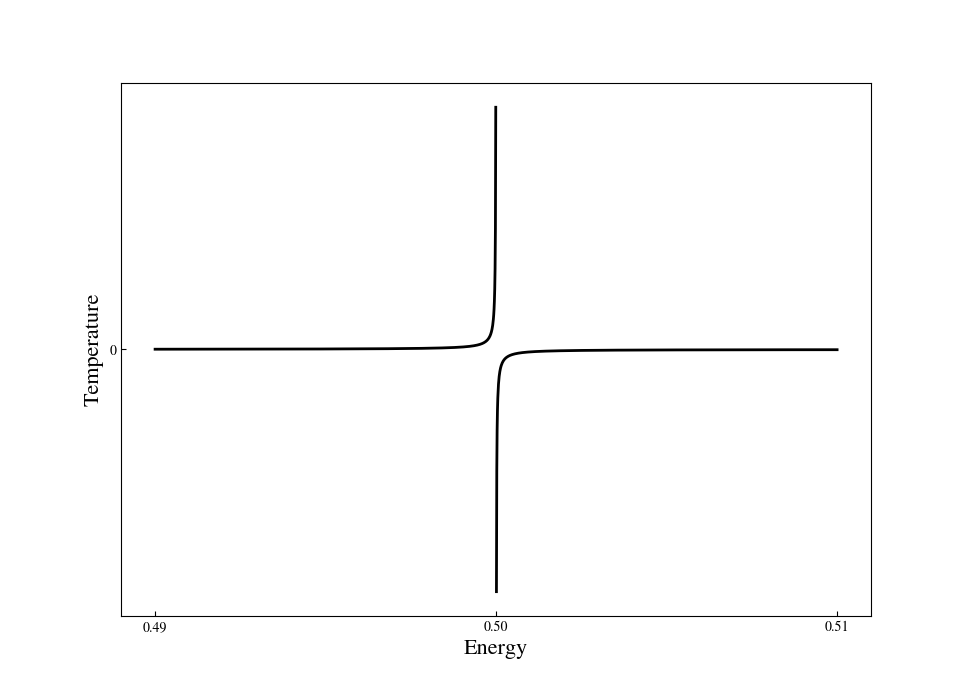
\includegraphics[scale=0.65]{images/temperature_TLS.png}
    \caption{The plot reports the temperature as a function of the energy in a two-levels system. When there are more excited particles than those in the lower state (Energy $> 0.5$), the system exhibits negative absolute temperatures.}
    \label{fig:temperature_TLS}
\end{figure}
Let us recall what we mentioned at the end of \hyperref{sec:temperature}{section 2}: a system whose maximum energy state is allowed by only one or few microstates may exhibit a decreasing entropy as a function of the energy, hence admitting negative temperatures. This is 
exactly the case of a TLS for which the maximum energy state corresponds to exactly one precise microstate, that is when all the particles are in the excited state. This of course corresponds to a null entropy. Analogously, the same happens at the minimum energy for which there is only 
one corresponding microstate and the entropy is null. For all the other states the entropy is non-zero and is given by formula \ref{eq:TLS_entropy_N_approx}. The whole expressions as a function of the energy can be easilly obtained by \ref{eq:TLS_entropy_N} by multiplying and diving by $\epsilon$ both inside and outside the logarithm
\begin{equation*}
    S(E, N) / k_B = N \ln\left(\frac{N\epsilon}{N\epsilon - E}\right) + \frac{E}{\epsilon} \ln\left(\frac{N\epsilon - E}{\epsilon}\right)
\end{equation*}
and is reported in figure \ref{fig:TLS_entropy_E}. \\
\begin{figure}
    \centering 
    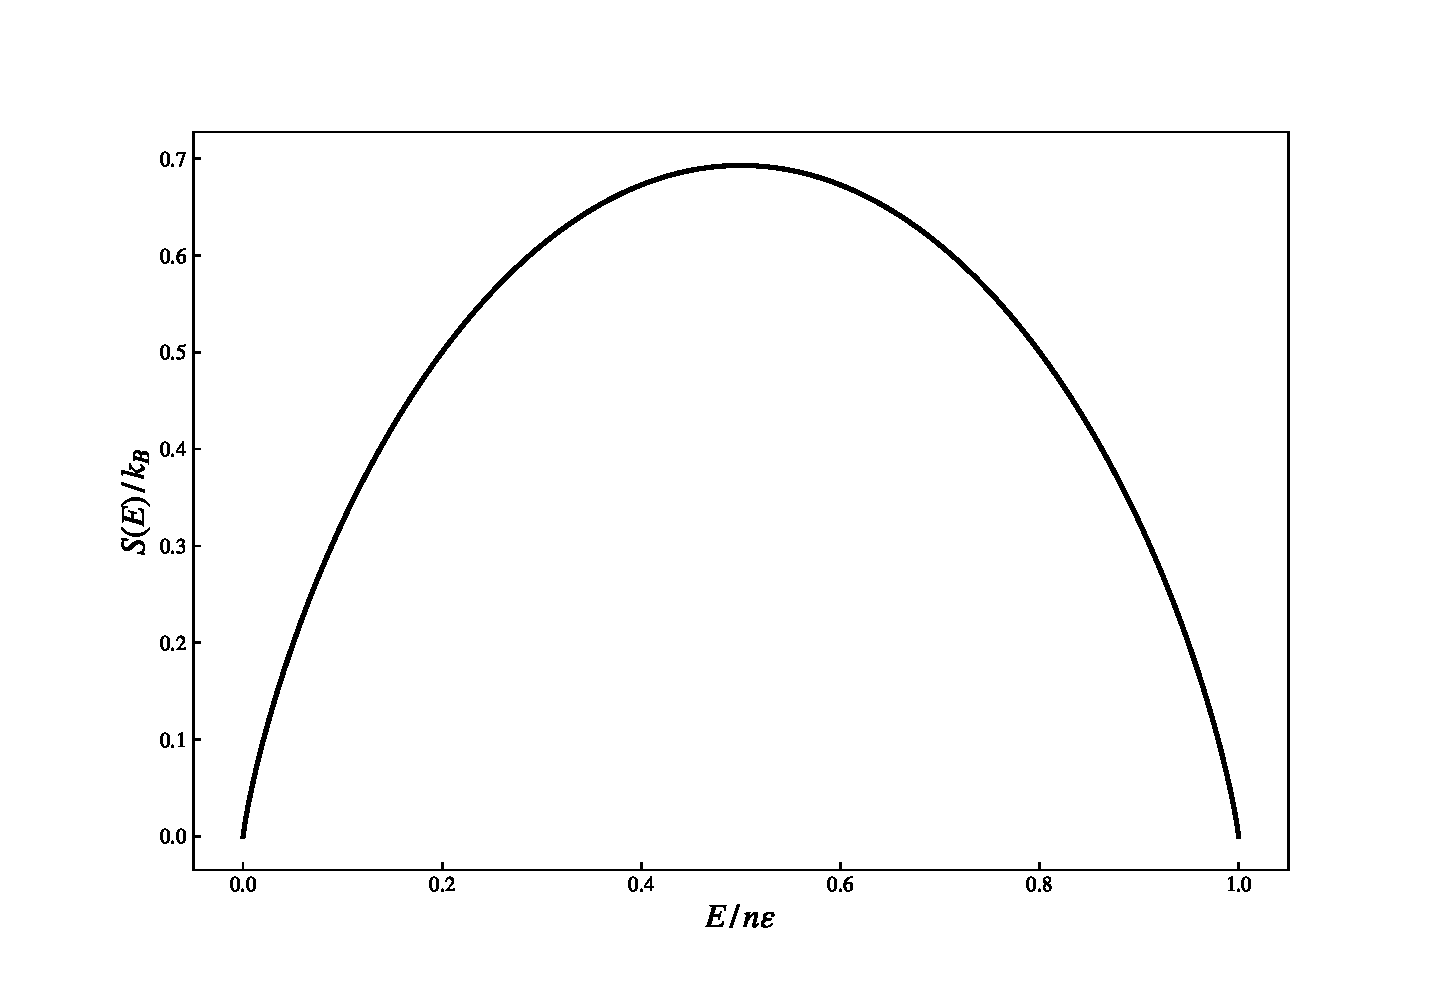
\includegraphics[scale=0.65]{images/entropy_TLS.eps}
    \caption{Entropy of a TLS as a function of the energy.}
    \label{fig:TLS_entropy_E}
\end{figure}
Let us formalize this insight in the next section.
\subsubsection*{Ramsey's criteria}
Ramsey %\cite{Ramsey}} 
provided 3 conditions under which a thermodynamic system exhibits negative temperatures
\begin{enumerate}
    \item \emph{The various elements of the thermodynamic system under analysis must be at equilibrium each other}. \\
    This condition must be verified in order to define a temperature for the whole system.
    \item \emph{There must be an upper bound on the energy of the system} \\
    In fact it is known from statistical mechanics that the probability (or probability density) for the system to be in a state of energy $E$ is 
    \begin{equation}
        p(E) \propto e^{-\beta E}
        \label{eq:probability_ramsey}
    \end{equation}
    where $\beta = 1/k_BT$. If negative temperatures are admitted by the system and the latter does not admit an upper bound on the energy, the exponential factor in equation \ref{eq:probability_ramsey}
    becomes infinitely large for increasing energy. This means that if the system admits negative temperature, the higher the energy, the higher the probability of the system to be in that state. The most probable state 
    would then be the one at infinite energy making the other states negligible. Clearly, an infinite amount of energy cannot be put into the system, meaning that such a system cannot exists.
    \item \emph{The thermodynamic system under analysis must be thermally isolated from other systems that do not satisfy the above conditions}. \\
    In good approximation one can think that the time required to reach equilibrium between the elements of the system is small compared to the time of interaction
    between the system and the environment or another system.
\end{enumerate}
The above conditions are all satisfied by the TLS described above. Indeed it admits negative temperatures.